

\section{Distintos K-Fold}

En este nuevo experimento vamos a querer encontrar la relación que se encuentra entre el tamaño de $K$-fold que utilizemos y los resultados óptimos conseguidos. De esta manera usaremos nuevamente el k y el $\alpha$ que nos dio mejores resultados, pero esta vez variaremos el $K \in {2,5,8,11,15}$ de Cross validation entre los siguientes parametros . Estos fueron elegidos de esta manera ya que si utilizabamos mayores $K$ el experimento tardaria mucho mas en terminar su ejecución


\subsection{Hipótesis}

Lo que creemos que ocurrirá, a partir de los resultados obtenidos en el experimento anterior, es que con $K$ mayores el resultado se ira mejorando. La razón por la que tomamos esta hipótesis sera que a medida que sea mas grande el $K$, el set de entrenamiento será mayor. Por esto mismo se tendra mas información al decidir a que clase pertenece cada imágen.

\subsection{Resultados}


\begin{figure}
	\centering
	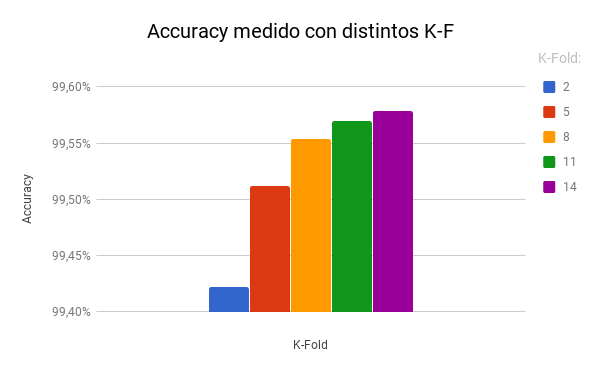
\includegraphics[width=\textwidth]{graficos/Distintos_kfold.png}
	\caption{Accuracy en función de distintos K-Fold}
	\label{fig:distintos_kfold}
\end{figure}

Finalmente se logro el resultado esperado. Como se ve en los gráficos, los resultados son mejores a partir de tener $K$ mayores, y esto se debe a que a medida que el $K$ se agranda, también se agranda la cantidad de datos de entrenamiento que se toman.

Por lo tanto de aquí podemos decir que con estos valores y utilizando toda la base de entrenamiento como tal, podemos obtener el mejor resultado, este sera el que utilizaremos en el torneo del sitio web kaggle.
